% !TEX TS-program = pdflatex
% !TEX encoding = UTF-8 Unicode

% This is a simple template for a LaTeX document using the "article" class.
% See "book", "report", "letter" for other types of document.

\documentclass[12pt]{article} % use larger type; default would be 10pt

\usepackage[utf8]{inputenc} % set input encoding (not needed with XeLaTeX)

%%% Examples of Article customizations
% These packages are optional, depending whether you want the features they provide.
% See the LaTeX Companion or other references for full information.

%%% PAGE DIMENSIONS
\usepackage[top=1.15in, bottom=0.75in, left=1.00in, right=1.00in]{geometry}
\geometry{a4paper} % or letterpaper (US) or a5paper or....
% \geometry{margin=2in} % for example, change the margins to 2 inches all round
% \geometry{landscape} % set up the page for landscape
%   read geometry.pdf for detailed page layout information

\usepackage{graphicx} % support the \includegraphics command and options

% \usepackage[parfill]{parskip} % Activate to begin paragraphs with an empty line rather than an indent

%%% PACKAGES
\usepackage{booktabs} % for much better looking tables
\usepackage{array} % for better arrays (eg matrices) in maths
\usepackage{paralist} % very flexible & customisable lists (eg. enumerate/itemize, etc.)
\usepackage{verbatim} % adds environment for commenting out blocks of text & for better verbatim
\usepackage{subfigure} % make it possible to include more than one captioned figure/table in a single float
% These packages are all incorporated in the memoir class to one degree or another...

%%% HEADERS & FOOTERS
\usepackage{fancyhdr} % This should be set AFTER setting up the page geometry
\pagestyle{fancy} % options: empty , plain , fancy
\renewcommand{\headrulewidth}{0pt} % customise the layout...
\lhead{}\chead{}\rhead{}
\lfoot{}\cfoot{\thepage}\rfoot{}

%%% SECTION TITLE APPEARANCE
\usepackage{sectsty}
\allsectionsfont{\sffamily\mdseries\upshape} % (See the fntguide.pdf for font help)
% (This matches ConTeXt defaults)

%%% ToC (table of contents) APPEARANCE
\usepackage[nottoc,notlof,notlot]{tocbibind} % Put the bibliography in the ToC
\usepackage[titles,subfigure]{tocloft} % Alter the style of the Table of Contents
\renewcommand{\cftsecfont}{\rmfamily\mdseries\upshape}
\renewcommand{\cftsecpagefont}{\rmfamily\mdseries\upshape} % No bold!
\usepackage[UTF8]{ctex}
\usepackage{fancyhdr}
\usepackage{enumerate}
\usepackage{indentfirst}
\usepackage{extramarks}
\usepackage{multirow}
\usepackage{titling}
\usepackage{amssymb}
\usepackage{amsmath}

%%% END Article customizations

%%% The "real" document content comes below...

\title{\textbf{Y86 Assembly IDE 使用说明}}
\author{周芯怡 17307130354\\张作柏 17300240035}
\date{\today}
%\date{} % Activate to display a given date or no date (if empty),
         % otherwise the current date is printed 

\begin{document}
\begin{sloppypar}
\maketitle

\section{简介}

Y86 Assembly IDE提供书写Y86汇编代码与动态调试的基本功能:
\begin{itemize}
\item 支持将汇编代码和指令码以.yo文件的形式输出
\item 支持运行中跳转至任意语句
\item 支持设置断点
\item 支持设置、监视特定值
\item 强大的help功能
\end{itemize}

Y86汇编IDE开发基于Django框架,运行需要安装Python 2.7与Django 1.10。

%%%%%%%%%%%%%%%%%%%%%%%%%%%%%%%%%%%%%%%%%%%%%%%%%%%%%%%%%%%
%% Figure  1
%%%%%%%%%%%%%%%%%%%%%%%%%%%%%%%%%%%%%%%%%%%%%%%%%%%%%%%%%%%
%\begin{figure}[htbp]
%\begin{center}
%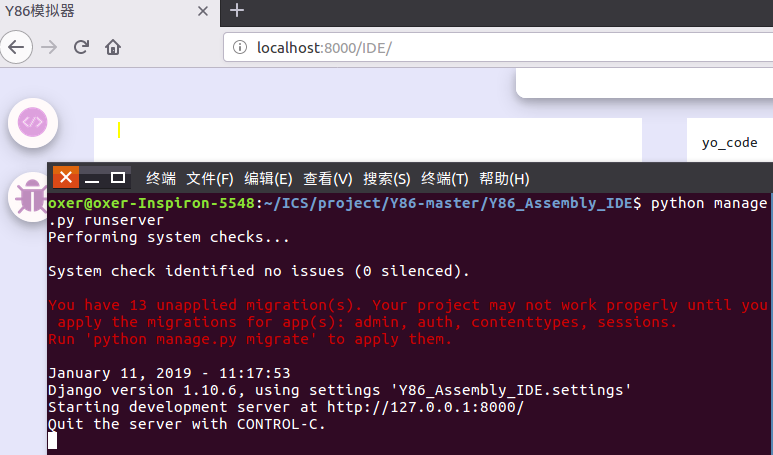
\includegraphics[width=.6\linewidth]{asset/1.png}
%\end{center}
%\end{figure}
%%%%%%%%%%%%%%%%%%%%%%%%%%%%%%%%%%%%%%%%%%%%%%%%%%%%%%%%%%%

使用时,需在Y86/Y86\_Assembly\_IDE目录下打开命令行,输入指令 python manage.py runserver 。运行成功后,打开浏览器,输入地址 http://localhost:8000/IDE即可进入IDE界面。

\clearpage
\section{界面说明}

\subsection{代码界面}

%%%%%%%%%%%%%%%%%%%%%%%%%%%%%%%%%%%%%%%%%%%%%%%%%%%%%%%%%%
% Figure  2
%%%%%%%%%%%%%%%%%%%%%%%%%%%%%%%%%%%%%%%%%%%%%%%%%%%%%%%%%%
\begin{figure}[htbp]
\begin{center}
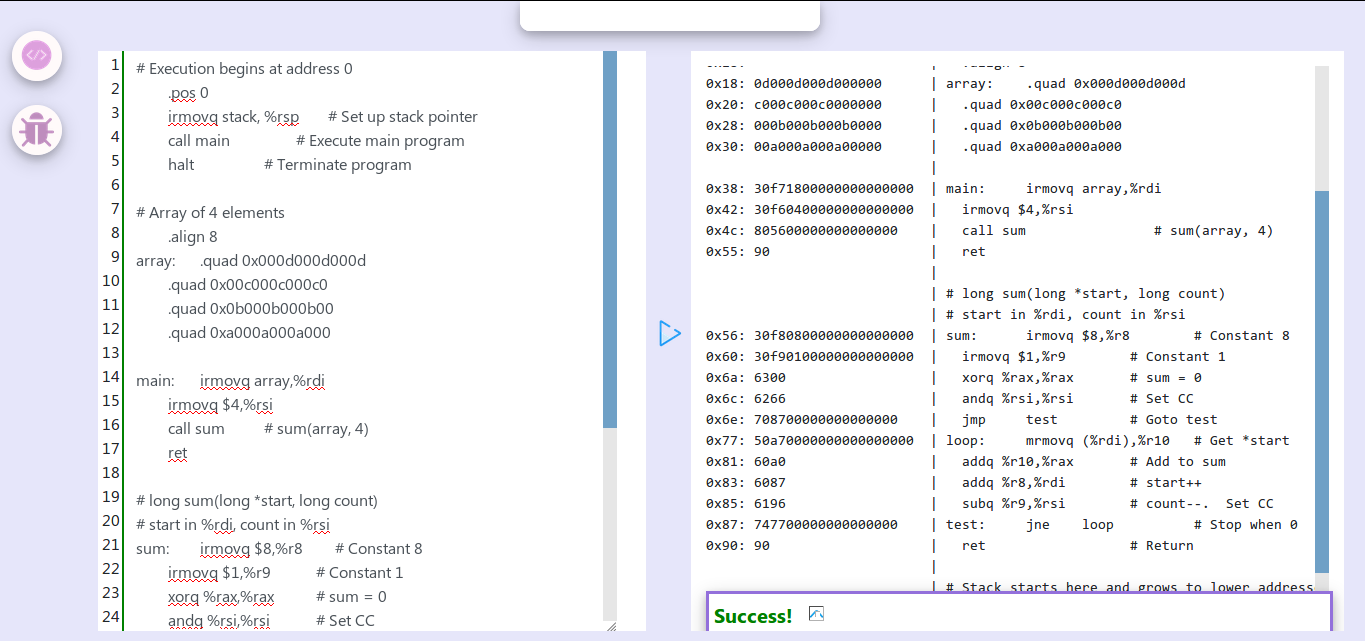
\includegraphics[width=\linewidth]{asset/2.png}
\end{center}
\end{figure}
%%%%%%%%%%%%%%%%%%%%%%%%%%%%%%%%%%%%%%%%%%%%%%%%%%%%%%%%%%

如上图,左侧为代码框,用于书写汇编代码,右侧为编译成功后的.yo代码。

为方便阅读,书写代码时会自动添加行号。未进行编译时,左侧边框为黄色,点击编译按钮后,边框变为绿色,表示已完成编译。


%%%%%%%%%%%%%%%%%%%%%%%%%%%%%%%%%%%%%%%%%%%%%%%%%%%%%%%%%%%
%% Figure  3 & 4
%%%%%%%%%%%%%%%%%%%%%%%%%%%%%%%%%%%%%%%%%%%%%%%%%%%%%%%%%%%
%\begin{figure}[htbp]
%\centering
%\subfigure{
%\begin{minipage}[t]{0.4\linewidth}
%\centering
%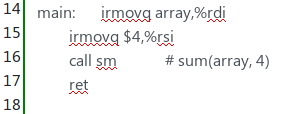
\includegraphics[width=\linewidth]{asset/3.png}
%\end{minipage}%
%}%
%\subfigure{
%\begin{minipage}[t]{0.6\linewidth}
%\centering
%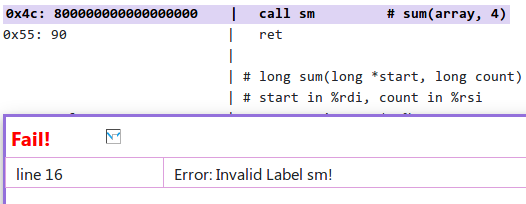
\includegraphics[width=.8\linewidth]{asset/4.png}
%\end{minipage}%
%}%
%\centering
%\end{figure}
%%%%%%%%%%%%%%%%%%%%%%%%%%%%%%%%%%%%%%%%%%%%%%%%%%%%%%%%%%%

右下方{\bf Error Info}一栏显示编译信息:编译成功时,显示Success;编译失败时,显示Failed,并弹出错误列表。错误列表将显示错误的行号,并返回详细错误。双击该错误,可使.yo代码中相应行高亮显示。

\clearpage
\subsection{Debug界面}

%%%%%%%%%%%%%%%%%%%%%%%%%%%%%%%%%%%%%%%%%%%%%%%%%%%%%%%%%%
% Figure  6
%%%%%%%%%%%%%%%%%%%%%%%%%%%%%%%%%%%%%%%%%%%%%%%%%%%%%%%%%%
\begin{figure}[htbp]
\begin{center}
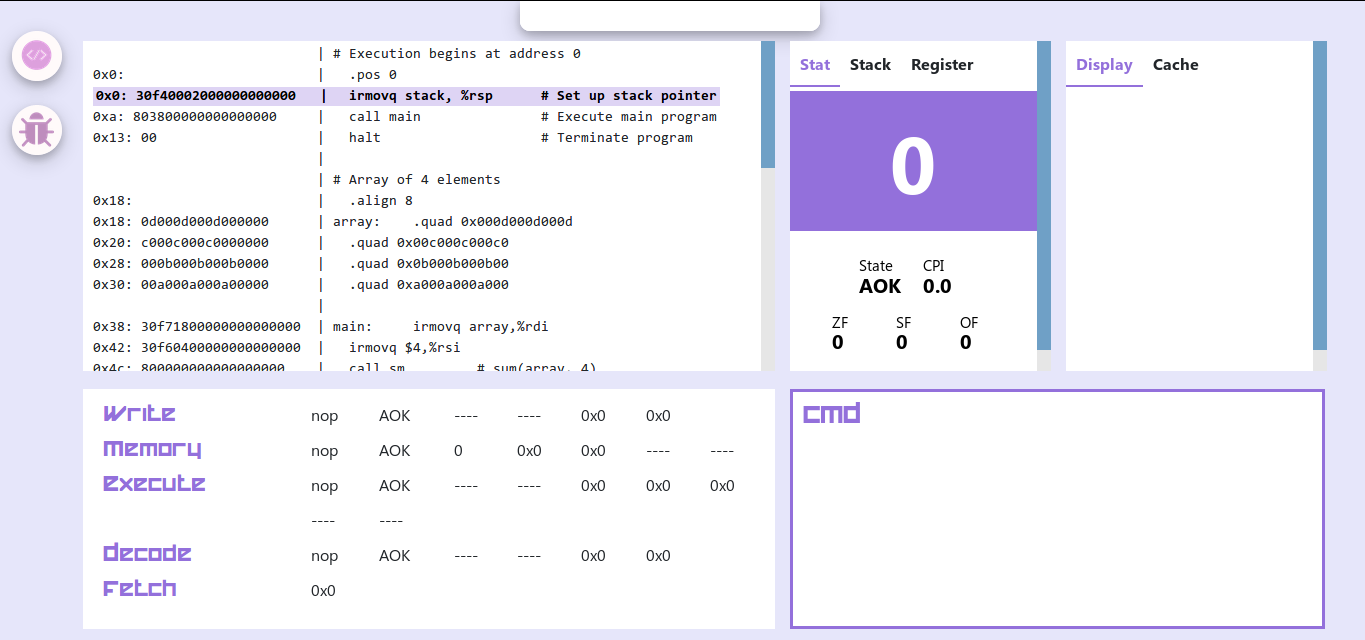
\includegraphics[width=\linewidth]{asset/6.png}
\end{center}
\end{figure}
%%%%%%%%%%%%%%%%%%%%%%%%%%%%%%%%%%%%%%%%%%%%%%%%%%%%%%%%%%

点击页面左侧图标可切换至Debug界面。

%%%%%%%%%%%%%%%%%%%%%%%%%%%%%%%%%%%%%%%%%%%%%%%%%%%%%%%%%%%
%% Figure  9
%%%%%%%%%%%%%%%%%%%%%%%%%%%%%%%%%%%%%%%%%%%%%%%%%%%%%%%%%%%
%\begin{figure}[htbp]
%\begin{center}
%
\includegraphics[width=.5\linewidth]{asset/9.png}
%\end{center}
%\end{figure}
%%%%%%%%%%%%%%%%%%%%%%%%%%%%%%%%%%%%%%%%%%%%%%%%%%%%%%%%%%%

页面{\bf 上方}为指令输入框,用于输入指令。

%%%%%%%%%%%%%%%%%%%%%%%%%%%%%%%%%%%%%%%%%%%%%%%%%%%%%%%%%%%
%% Figure  7
%%%%%%%%%%%%%%%%%%%%%%%%%%%%%%%%%%%%%%%%%%%%%%%%%%%%%%%%%%%
%\begin{figure}[htbp]
%\begin{center}
%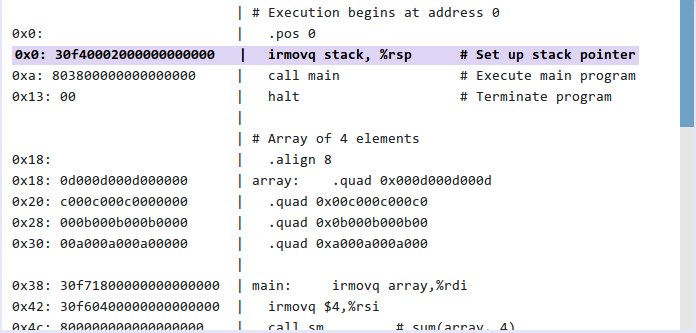
\includegraphics[width=.9\linewidth]{asset/7.png}
%\end{center}
%\end{figure}
%%%%%%%%%%%%%%%%%%%%%%%%%%%%%%%%%%%%%%%%%%%%%%%%%%%%%%%%%%%

{\bf 左上方}为.yo代码框。汇编代码编译成功后,.yo代码会自动同步到此处。代码运行过程中,会高亮当前行,清晰显示代码运行过程。

%\clearpage
%
%%%%%%%%%%%%%%%%%%%%%%%%%%%%%%%%%%%%%%%%%%%%%%%%%%%%%%%%%%%
%% Figure  8 & 10
%%%%%%%%%%%%%%%%%%%%%%%%%%%%%%%%%%%%%%%%%%%%%%%%%%%%%%%%%%%
%\begin{figure}[htbp]
%\centering
%\subfigure{
%\begin{minipage}[t]{0.55\linewidth}
%\centering
%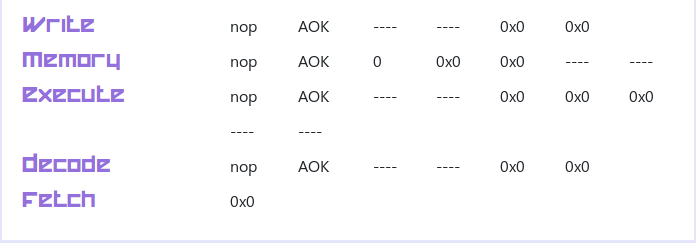
\includegraphics[width=0.95\linewidth]{asset/8.png}
%\end{minipage}%
%}%
%\subfigure{
%\begin{minipage}[t]{0.45\linewidth}
%\centering
%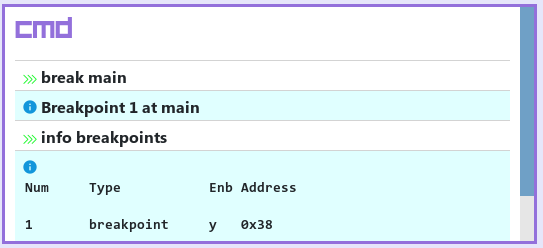
\includegraphics[width=0.95\linewidth]{asset/10.png}
%\end{minipage}%
%}%
%\centering
%\end{figure}
%%%%%%%%%%%%%%%%%%%%%%%%%%%%%%%%%%%%%%%%%%%%%%%%%%%%%%%%%%%

{\bf 左下方}为流水线寄存器的信息显示,将鼠标放在数字上,可显示对应的含义。指令执行过程中,五个Stage图标会闪烁,亮起表示正在执行,熄灭表示执行完毕,以此来可视化并行过程。



{\bf 右下方}为{\bf CMD}窗口,返回指令执行信息,可显示输入指令及返回的运行结果。

%%%%%%%%%%%%%%%%%%%%%%%%%%%%%%%%%%%%%%%%%%%%%%%%%%%%%%%%%%%
%% Figure  11 & 12 & 13
%%%%%%%%%%%%%%%%%%%%%%%%%%%%%%%%%%%%%%%%%%%%%%%%%%%%%%%%%%%
%\begin{figure}[htbp]
%\centering
%\subfigure{
%\begin{minipage}[t]{0.3\linewidth}
%\centering
%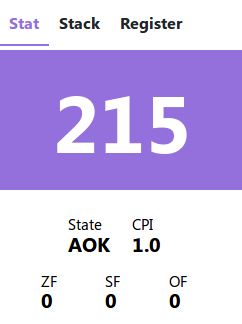
\includegraphics[width=0.95\linewidth]{asset/11.png}
%\end{minipage}%
%}%
%\subfigure{
%\begin{minipage}[t]{0.4\linewidth}
%\centering
%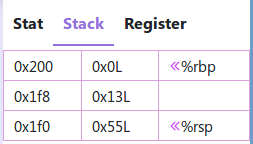
\includegraphics[width=0.95\linewidth]{asset/12.png}
%\end{minipage}%
%}%
%\subfigure{
%\begin{minipage}[t]{0.3\linewidth}
%\centering
%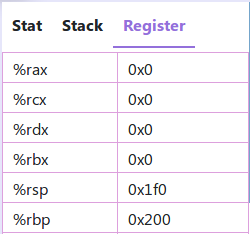
\includegraphics[width=0.95\linewidth]{asset/13.png}
%\end{minipage}%
%}%
%\centering
%\end{figure}
%%%%%%%%%%%%%%%%%%%%%%%%%%%%%%%%%%%%%%%%%%%%%%%%%%%%%%%%%%%

{\bf 正中}为运行状态窗口,可分别显示运行的状态(Cycle数,Status,CPI,条件码)、栈中元素、寄存器的值。

%%%%%%%%%%%%%%%%%%%%%%%%%%%%%%%%%%%%%%%%%%%%%%%%%%%%%%%%%%%
%% Figure  14 & 15
%%%%%%%%%%%%%%%%%%%%%%%%%%%%%%%%%%%%%%%%%%%%%%%%%%%%%%%%%%%
%\begin{figure}[htbp]
%\centering
%\subfigure{
%\begin{minipage}[t]{0.4\linewidth}
%\centering
%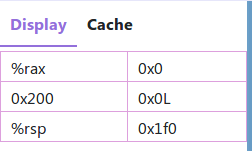
\includegraphics[width=0.9\linewidth]{asset/14.png}
%\end{minipage}%
%}%
%\subfigure{
%\begin{minipage}[t]{0.3\linewidth}
%\centering
%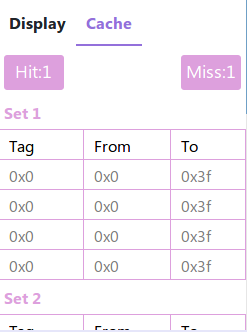
\includegraphics[width=0.9\linewidth]{asset/15.png}
%\end{minipage}%
%}%
%\centering
%\end{figure}
%%%%%%%%%%%%%%%%%%%%%%%%%%%%%%%%%%%%%%%%%%%%%%%%%%%%%%%%%%%

{\bf 右上方}为显示窗口,可观察设置为Display的变量与Cache当前的存储信息。

\clearpage
\section{指令说明}

\subsection{\#Step指令集}

\begin{table}[h]
\begin{tabular}{|c|l|}
\hline
{\bf 指令} & {\bf 说明} \\ 
\hline
\multirow{4}{*}{step} & 格式: step [N] \\
 & 不带参数时,执行下一个指令 \\
 & 带参数时,参数[N]表示前进N步(除非程序中止) \\
 & 可缩写为s \\ 
\hline
\multirow{4}{*}{next} & 格式: next [N] \\
 & 不带参数时,执行下一个指令,不会进入子函数 \\
 & 带参数时,参数[N]表示前进N步(除非程序中止) \\
 & 可缩写为n \\ 
\hline
\multirow{3}{*}{continue} & 格式: continue \\
 & 继续执行当前程序,直到遇到断点或中止信号 \\
 & 可缩写为c \\
\hline
\multirow{2}{*}{finish} & 格式: finish \\
 & 执行当前程序,直到退出当前函数 \\
\hline
\end{tabular}
\end{table}

\subsection{\#Jump指令集}

\begin{table}[h]
\begin{tabular}{|c|l|}
\hline
{\bf 指令} & {\bf 说明} \\ 
\hline
\multirow{3}{*}{jump} & 格式: jump $\langle location\rangle$ \\
 & 令PC跳至位置$\langle location\rangle$处 \\
 & $\langle location\rangle$可以是指令地址,可以是合法的label \\
\hline
\multirow{2}{*}{return} & 格式: return \\
 & 直接跳出当前函数。 \\
\hline
\multirow{2}{*}{call} & 格式: call $\langle label\rangle$ \\
 &  直接调用label函数。 \\
\hline
\end{tabular}
\end{table}

\clearpage
\subsection{\#Breakpoints指令集}

\begin{table}[!hbp]
\resizebox{\textwidth}{45mm}{
\begin{tabular}{|c|l|}
\hline
{\bf 指令} & {\bf 说明} \\ 
\hline
\multirow{2}{*}{break} & 格式: break $\langle location\rangle$ \\
 & 在位置$\langle location\rangle$处设置断点。 \\
\hline
\multirow{2}{*}{info breakpoints} & 格式: info breakpoints \\
 & 输出所有用户设置的未被删除的断点信息,包括断点编号、断点状态、断点位置。 \\
\hline
\multirow{3}{*}{enable} & 格式: enable $\langle NUM\rangle$ \\
 & 使编号为$\langle NUM\rangle$的断点重新发挥作用,相对指令disable。 \\
 & 若不带任何参数,则恢复所有断点。 \\
\hline
\multirow{3}{*}{disable} & 格式: disable $\langle NUM\rangle$ \\
 & 使编号为$\langle NUM\rangle$的断点失去作用,即遇到该断点时不在停止,相对指令enable。 \\
 & 若不带任何参数,则使所有断点失去作用。 \\
\hline
\multirow{3}{*}{delete} & 格式: delete $\langle NUM\rangle$ \\
 & 删除编号为$\langle NUM\rangle$的断点,连其编号一同移除,即之后不再有编号为$\langle NUM\rangle$的断点。 \\
 & 若不带任何参数,则删除所有断点。 \\
\hline
\end{tabular}}
\end{table}

\subsection{\#Display指令集}

\begin{table}[!hbp]
\resizebox{\textwidth}{55mm}{
\begin{tabular}{|c|l|}
\hline
{\bf 指令} & {\bf 说明} \\ 
\hline
\multirow{9}{*}{display} & 格式: display $\langle EXP\rangle$ \\
 & 在Display框中实时显示EXP变量的值。 \\
 & 几种EXP的格式: \\
 & REG $\langle REGNAME\rangle$ 例:REG \%rax \\
 & 显示系统寄存器$\langle REGNAME\rangle$的值,注意$\langle REGNAME\rangle$必须以'\%'开头。 \\
 & MEM $\langle ADDR\rangle$    例:MEM 0x200 \\
 & 显示内存地址$\langle ADDR\rangle$中的值,注意$\langle ADDR\rangle$必须是十六进制表示。 \\
 & STACK $\langle NUMID\rangle$ 例:STACK 0 \\
 & 显示系统栈顶第$\langle NUMID\rangle$个元素的值,下标从0开始,注意$\langle NUMID\rangle$必须是十进制表示。 \\
\hline
\multirow{9}{*}{undisplay} & 格式: undisplay $\langle EXP\rangle$ \\
 & 在Display框中取消显示EXP变量的值。 \\
 & 几种EXP的格式: \\
 & REG $\langle REGNAME\rangle$ 例:REG \%rax \\
 & 显示系统寄存器$\langle REGNAME\rangle$的值,注意$\langle REGNAME\rangle$必须以'\%'开头。 \\
 & MEM $\langle ADDR\rangle$    例:MEM 0x200 \\
 & 显示内存地址$\langle ADDR\rangle$中的值,注意$\langle ADDR\rangle$必须是十六进制表示。 \\
 & STACK $\langle NUMID\rangle$ 例:STACK 0 \\
 & 显示系统栈顶第$\langle NUMID\rangle$个元素的值,下标从0开始,注意$\langle NUMID\rangle$必须是十进制表示。 \\
\hline
\end{tabular}}
\end{table}

\clearpage
\subsection{\#I/O指令集}

\begin{table}[!hbp]
\resizebox{\textwidth}{45mm}{
\begin{tabular}{|c|l|}
\hline
{\bf 指令} & {\bf 说明} \\ 
\hline
\multirow{2}{*}{write} & 格式: write $\langle FILENAME\rangle$ \\
 & 将指令码与汇编代码以.yo文件的格式写入文件$\langle FILENAME\rangle$中。 \\
\hline
\multirow{2}{*}{list} & 格式: list \\
 & 将指令码与汇编代码以.yo文件的格式显示在屏幕上。 \\
\hline
\multirow{5}{*}{load} & 格式: load $\langle FILENAME\rangle$ \\
 & 清除之前所有的代码和状态。 \\
 & 从$\langle FILENAME\rangle$中加载指令码和汇编码,$\langle FILENAME\rangle$必须是.yo文件或.ys文件。 \\
 & 当加载.yo类型文件时,可直接从中提取指令码。 \\
 & 当加载.ys类型文件时,调用YAS生成指令码,并记录所有label。 \\
\hline
\multirow{4}{*}{read} & 格式: read [Enter] \\
 & $\langle Assembly Code\rangle$ \\
 & [Enter] \\
 & 动态输入汇编代码,附加在当前代码集合之后,可以调用之前的label,可以新建label。 \\
\hline
\end{tabular}}
\end{table}

\subsection{\#Others指令集}

\begin{table}[!hbp]
\resizebox{\textwidth}{55mm}{
\begin{tabular}{|c|l|}
\hline
{\bf 指令} & {\bf 说明} \\ 
\hline
\multirow{9}{*}{set} & 格式: set $\langle EXP\rangle$ $\langle value\rangle$ \\
 & 几种EXP的格式: \\
 & REG $\langle REGNAME\rangle$ 例:REG \%rax \\
 & 显示系统寄存器$\langle REGNAME\rangle$的值,注意$\langle REGNAME\rangle$必须以'\%'开头。 \\
 & MEM $\langle ADDR\rangle$    例:MEM 0x200 \\
 & 显示内存地址$\langle ADDR\rangle$中的值,注意$\langle ADDR\rangle$必须是十六进制表示。 \\
 & STACK $\langle NUMID\rangle$ 例:STACK 0 \\
 & 显示系统栈顶第$\langle NUMID\rangle$个元素的值,下标从0开始,注意$\langle NUMID\rangle$必须是十进制表示。 \\
 & 将表达式$\langle EXP\rangle$指定的值设为$\langle value\rangle$。 \\
\hline
\multirow{2}{*}{clear} & 格式: clear \\
 & 清除当前所有代码和状态。 \\
\hline
\multirow{5}{*}{help} & 格式: help $\langle CMD\rangle$ \\
 & 显示$\langle CMD\rangle$指令的使用说明。 \\
 & 当不加参数时,显示所有指令组。 \\
 & 当$\langle CMD\rangle$为指令组时,显示该指令组内的所有指令简介。 \\
 & 当$\langle CMD\rangle$为某个指令时,显示该指令的使用方法。 \\
\hline
\multirow{2}{*}{quit} & 格式: quit \\
 & 退出Y86 Assembly IDE。 \\
\hline
\end{tabular}}
\end{table}

\clearpage
\section{注意事项}

\begin{itemize}
\item 载入.yo文件时,不支持任何label操作。因为载入时直接读取指令码,所以无法对应label。
\item 直接输入回车[Enter]时,会执行上一条指令。
\item 载入文件时,会自动清除之前的所有代码与状态。
\item 支持\#和/**/两种注释格式,暂不支持分行注释。
\end{itemize}

\end{sloppypar}
\end{document}
